\documentclass[12pt]{article}
\usepackage[a4paper, margin=.30in]{geometry}
%\usepackage{array}
\usepackage{graphicx, subfig, wrapfig ,multicol, color }
\setlength{\columnseprule}{1pt}
\def\columnseprulecolor{\color{blue}}
\usepackage[mathscr]{euscript}
\newcommand\headerMe[2]{\noindent{}#1\hfill#2}









\begin{document}

\headerMe{Royaume du Maroc}{année scolaire \emph{2021-2022}}\\
\headerMe{Ministère de l'Éducation nationale, }{  Professeur :\emph{Zakaria Haouzan}}\\
\headerMe{du Préscolaire et des Sports}{Établissement : \emph{Lycée SKHOR qualifiant}}\\

\begin{center}
Devoir surveillé N°1 \\
    Filière 1Bac Sciences Expérimentales\\
Durée 2h00
\\
 %   \vspace{.2cm}
%\hrulefill
%\Large{Chimie 6pts}
%\hrulefill\\
 %   \emph{Les deux parties sont indépendantes}
\end{center}
%end Headerss------------------------


%__________________Chimie ______________________-
%%%%%%%+_+_+_+_+_+_+_+_+_Partie1


\begin{multicols}{2}
    [
        \section*{Questions du cours: Choisir la bonne réponse. (5 pts)}
    ]

\begin{enumerate}
  \item La relation entre la vitesse linéaire et la vitesse angulaire est :
      \begin{enumerate}
          \item $V = R.\omega$\sloppy
          \item $\omega = R.V$\nolinebreak
          \item $R = V.\omega$
      \end{enumerate}

  \item  Unité de la puissance d’une force est :
      \begin{enumerate}
          \item[] a)Joule \hspace{1cm}  b)Newton  \hspace{1cm}c)Watt
      \end{enumerate}

     \item  La concentration massique d'un soluté dans une solution s'exprime en :
      \begin{enumerate}
          \item $L.g^{-1}$
          \item $g.L^{-1}$
          \item $g$
          \item $L$
      \end{enumerate}
        \vspace{1cm}
 \item  Un solide est animé d’un mouvement de translation rectiligne uniforme. Il est soumis à deux
forces constantes :
      \begin{enumerate}
          \item  Le travail de chacune des forces est nul 
          \item Le travail de la somme des forces est nul
          \item La somme des travaux de ces deux forces n’est pas nulle
      \end{enumerate}

 \item  L'expression de la densité d'une espèce chimique X liquide ou solide vaut: 
      \begin{enumerate}
          \item $d = \rho_X \times \rho_{eau}$
          \item $d = \frac{m_X }{m_{eau}}$
          \item $d = \frac{\rho_{eau}}{\rho_{X}}$  
      \end{enumerate}

\end{enumerate}
\end{multicols}
%%%%%%%+_+_+_+_+_+_+_+_+_Partie2
%________________________________________
 \section*{Exercice 1 : solution de l’éthanol (3 Pts )}

Une solution de l’éthanol de volume V = 250ml contient une masse m = 1, 0g de l’éthanol.
\begin{enumerate}
\item Quelle est sa concentration massique ?\\\\
Pour déterminer la densité de l’éthanol , on mesure à vide la masse d’une fiole jaugée de 50,0ml , on trouve m1 = 61,7g . On introduit de l’éthanol jusquau niveau du trait de jauge et on mesure la masse de la fiole jaugée contenant de l’éthanol une deuxième fois , on trouve m2 = 101,2g .
\item Sachant que la masse de 50ml d’eau est égale à 50g ,calculer d la densité de l’éthanol
par rapport à l’eau .
\end{enumerate}
%_____________________________________PHYSIque Partie 22222____________________________________________________________________________
%\begin{center}
%    \vspace{.75cm}
%\hrulefill
%\Large{Physique 14pts}
%\hrulefill\\
%    \emph{Les trois parties sont indépendantes}
%\end{center}
%end Headerss------------------------

 \section*{Exercice 2 : Mouvement de Rotaion (5 pts)}
Un disque de diamètre D = 20 cm tourne autour d'un axe fixe $(\Delta)$, passe par son axe de symétrie. Le graphe ci-dessous montre les changements des abscisses angulaires du disque en fonction de temps.

\begin{enumerate}
\begin{figure}[h]
    \centering
    \subfloat[\centering figure 1 : disque de diamètre D tourne autour d'un axe fixe ]{{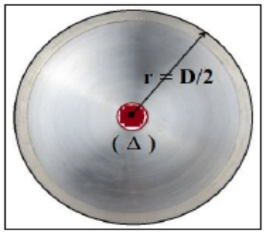
\includegraphics[width=4cm]{./img/img00.png} }}%
    \qquad
    \subfloat[\centering figure 2 : l'abscisse angulaire en fonction du temps t]{{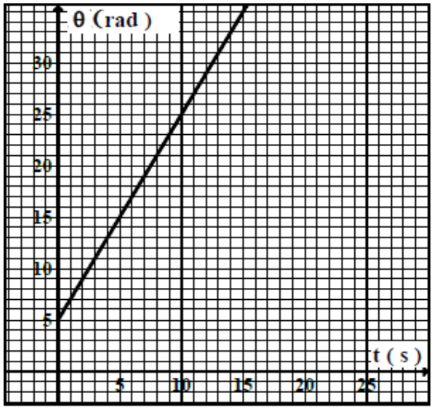
\includegraphics[width=5.5cm]{img/img01} }}%
\end{figure}
\item Quel est la nature du mouvement du disque ?
Justifier.
\item Déterminer la valeur de la vitesse angulaire .
\item Ecrire l'équation horaire $\theta(t) $du mouvement de disque .
\item Trouver l'équation horaire S(t).
    \item Quel est le nombre du tour qui fait le disque au
moment t=30s.
\item Déterminer la position du point M par rapport à
l'axe si sa vitesse Vm =0,1m/s.
\end{enumerate}



\section*{Exercice 3 : Le Travail d'une force constante (7pts)}
Un solide ponctuel (S) de masse $m = 0,4 Kg$ se
déplace avec une vitesse constante $v = 3 m.s^{-1}$ le long
d’un trajet ABC qui comporte deux phases :
\\- Une partie (AB) rectiligne de longueur AB = 15m
et incliné d’un angle $\alpha= 30^{\circ}$ par rapport à l’horizontale.
\\- une partie (BC) rectiligne et horizontale de
longueur BC = 10m 
\\-On donne g = 10N/Kg.
%\begin{wrapfigure}[4]{r}{0.3\textwidth}
  \begin{center}
    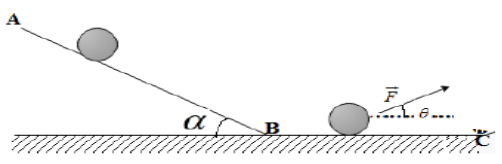
\includegraphics[width=0.5\textwidth]{./img/imgre00.png}
  \end{center}
%\end{wrapfigure}



\begin{enumerate}
    \item \underline{Mouvement du solide sur la partie (AB) :}
        \begin{enumerate}
                \item Faire un bilan des forces s’appliquant sur le solide (S) et les représenter sur le schéma.
                \item Calculer le travail du poids $\vec{P}$ du solide au cours du déplacement AB.
                \item  Calculer $\mathscr{P}_m(\vec{P})$ la puissance moyenne du poids de solide au cours du déplacement AB.
        \end{enumerate}
    \item \underline{Mouvement du solide sur la partie (BC) :}\\
Le solide est soumis à une force constante $\vec{F}$ d’intensité F=3N, faisant un angle $\theta = 60^{\circ}$ avec l’horizontal sur
la partie (BC).
        \begin{enumerate}
                
                \item Calculer le travail du poids $\vec{P}$ du solide et le travail de la force   $\vec{F}$ au cours du déplacement BC.
                    \item En appliquant le principe d’inertie, calculer le travail de la force de frottement.
                        \item Déduire la valeur de f l’intensité de la force frottement
        \end{enumerate}
\end{enumerate}

\end{document}
